\graphicspath{{./fig_Sample/}}


物理量モニタリング機能は,ユーザが指定した位置で指定した物理量をファイルに出力する機能である.
位置の指定には,ボクセルモデルのIDで指定する方法とXMLパラメータファイルで指定する2種類がある.
ここでは内部実装について説明する.

%%%
\section{物理量モニタリング機能API}
物理量モニタリング機能は,全モニタグループを管理するMonitorListクラス,
個々のモニターグループを管理するMonitorCompoクラス,
各モニタ点でのサンプリング機能を提供するSamplingクラスより構成される.

\begin{figure}[H]
\vspace{0.5cm}
\begin{center}
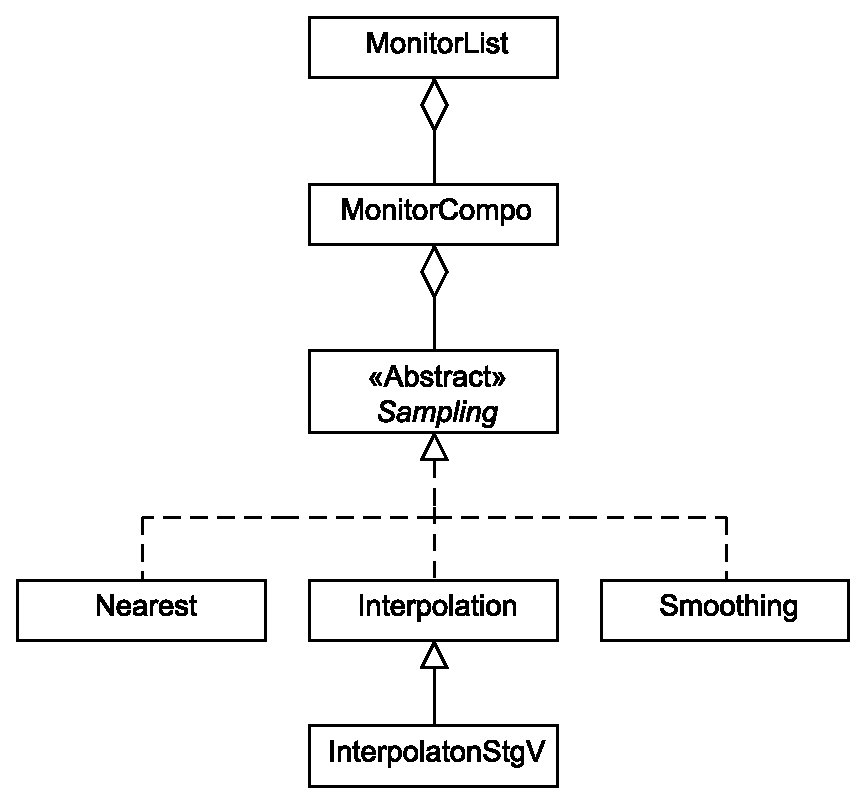
\includegraphics[width=0.7\textwidth]{Monitor.eps}
\caption{物理量モニタリング機能のクラス図}
\label{fig:monitor}
\end{center}
\end{figure}

MonitorListクラスおよびMonitorCompoクラスは,Parallel\_Nodeクラスを継承している.
Samplingクラスは抽象クラスで,
各モニタ点での実際のサンプリング計算は,Samplingクラスから継承された
Nearestクラス,Interpolationクラス,Smoothingクラスが担当する.
ソルバーから直接インスタンスされ操作されるのは,MonitorListクラスのみである.

\pagebreak
%%%
\subsection{MonitorListクラス公開メソッド}
%
\vspace{2mm}

\paragraph{必須パラメータのコピー}\mbox{}\\
モニタリング機能の管理およびサンプリング計算に必要なパラメータをコピーする.

\begin{table}[hp]
\begin{tabular}{ll}
{\tt bcd} & BCindex ID配列\\
{\tt g\_org} & グローバル領域基点座標\\
{\tt g\_lbx} & 領域サイズ\\
{\tt org} & ローカル領域基点座標\\
{\tt dx} & セル幅\\
{\tt lbx} & 領域サイズ\\
{\tt rs} & ローカルセルサイズ\\
{\tt gc} & ガイドセル数\\
{\tt refVelocity} & 代表速度\\
{\tt baseTemp} & 基準温度\\
{\tt diffTemp} & 代表温度差\\
{\tt refDensity} & 代表密度\\
{\tt refLength} & 代表長さ\\
{\tt basePrs} & 基準圧力\\
{\tt modeUnit} & 出力単位の指定フラグ(有次元,無次元)\\
{\tt unitTemp} & 温度の単位\\
{\tt modePrecision} & 精度のフラグ(単精度,倍精度)\\
{\tt unitPrs} & 圧力の単位\\
{\tt v00} & 座標系移動速度と成分\\
\end{tabular}
\end{table}

{\small
\begin{program}
void setControlVars(unsigned* bcd, SKL_REAL g_org[3], SKL_REAL g_lbx[3],
                  SKL_REAL org[3], SKL_REAL dx[3], SKL_REAL lbx[3],
                  unsigned rs[3], unsigned gc,
                  SKL_REAL refVelocity, SKL_REAL baseTemp, SKL_REAL diffTemp,
                  SKL_REAL refDensity, SKL_REAL refLength, SKL_REAL basePrs,
                  unsigned modeUnit, unsigned unitTemp,
                  unsigned modePrecision, unsigned unitPrs)
\end{program}
}

%
\paragraph{参照速度の指定}\mbox{}\\
引数{\tt v00[4]}には,参照格子系の速度と速度成分をもつ配列を指定する.
{\small
\begin{program}
void set_V00(SKL_REAL v00[4]) 
\end{program}
}

%
\paragraph{出力タイプの設定}\mbox{}\\
引数{\tt type}には,{\tt MonitorList::GATHER}(単一ファイル出力)
または{\tt MonitorList::DISTRIBUTE}(分散出力)を指定する.
{\small
\begin{program}
void setOutputType(OutputType type)
\end{program}
}

%
\paragraph{point\_setグループの登録}\mbox{}\\
ラベル文字列{\tt labelStr},モニタ対象物理量文字列のvector {\tt variables},
サンプリング方法文字列{\tt methodStr},
サンプリングモード文字列{\tt modeStr},
MonitorPoint構造体のvector {\tt pointSet}によりpoint\_setグループを登録する.
\pagebreak
{\small
\begin{program}
void setPointSet(const char* labelStr, vector<string>& variables,
                 const char* methodStr, const char* modeStr,
                 vector<MonitorCompo::MonitorPoint>& pointSet)
\end{program}
}
MonitorPoint構造体は,個々のモニタ点に対応した構造体である.

{\small
\begin{program}
struct MonitorPoint {
  Vec3r crd;      ///< モニタ点座標
  string label;   ///< モニタ点ラベル(コメント)
  MonitorPoint(const SKL_REAL v[3], const char* str) : crd(v), label(str) {}
  ~MonitorPoint() {}
};
\end{program}
}

%
\paragraph{lineグループの登録}\mbox{}\\
ラベル文字列{\tt labelStr},モニタ対象物理量文字列のvector {\tt variables},
サンプリング方法文字列{\tt methodStr},
サンプリングモード文字列{\tt modeStr},
線分端点座標{\tt from,to},分割数{\tt nDivision}
によりlineグループを登録する.
{\small
\begin{program}
void setLine(const char* labelStr, vector<string>& variables,
             const char* methodStr, const char* modeStr,
             SKL_REAL from[3], SKL_REAL to[3], int nDivision)
\end{program}
}

%
\paragraph{内部境界条件としてのモニタ指定の有無を調査}\mbox{}\\
サイズ{\tt nBC}のコンポーネント配列{\tt cmp}を調べ,
内部境界条件としてのモニタ指定があればtrueを返す.
{\small
\begin{program}
bool hasCellMonitor(CompoList* cmp, int nBC) 
\end{program}
}

%
\paragraph{内部境界条件としてのモニタ領域を登録}\mbox{}\\
サイズ{\tt nBC}のコンポーネント配列{\tt cmp}を参照して,
内部境界条件として指定されたモニタ領域を登録する.
{\small
\begin{program}
void setInnerBoundary(CompoList* cmp, int nBC)
\end{program}
}

%
\paragraph{サンプリング元となるデータ配列の登録}\mbox{}\\
速度変数配列{\tt v},
圧力変数配列{\tt p},
温度変数配列{\tt t}を登録.
{\small
\begin{program}
void setDataPtrs(SKL_REAL* v, SKL_REAL* p, SKL_REAL* t=NULL)
\end{program}
}

%
\paragraph{モニタ点位置情報の出力}\mbox{}\\
セルID配列{\tt id}に対して,
point\_setグループおよびlineグループのモニタ点を含むセルに対して
ID=255を書き込む.
{\small
\begin{program}
void write_ID(int* id)
\end{program}
}

%
\pagebreak
\paragraph{モニタリング情報を出力}\mbox{}\\
ファイルポインタ{\tt fp}に,
登録されたモニタリング設定情報を出力する.
{\small
\begin{program}
void printMonitorInfo(FILE* fp)
\end{program}
}

%
\paragraph{出力ファイルのオープン}\mbox{}\\
文字列{\tt str}にXMLコンフィギュレーションファイルの
OutputData要素のlog\_samplingで指定されたファイル名を渡すことにより,
各グループ用,各ノード用(分散出力時)のファイル名が生成され,オープンされる.
このメソッドは,出力タイプによらず,全プロセスから呼んでも問題ない.
{\small
\begin{program}
void openFile(const char* str)
\end{program}
}

%
\paragraph{サンプリング計算(point\_set, line)}\mbox{}\\
以下のメソッドにより,point\_setグループおよびlineグループの
各モニタ点でサンプリング計算を行う.
{\small
\begin{program}
void sampling()
\end{program}
}

%
\paragraph{サンプリング計算(内部境界条件)}\mbox{}\\
内部境界条件として指定されたモニタ領域のサンプリングには
次のメソッドを用いる.
このメソッドで,サンプリング結果のノード0への集計,モニタ領域内での平均,
速度の場合は法線ベクトルとの内積を計算し,コンポーネントcmpへの格納までを行う.
{\small
\begin{program}
void samplingInnerBoundary()
\end{program}
}

%
\paragraph{サンプリング結果の出力}\mbox{}\\
サンプリング時のステップ数{\tt step}およびソルバー内部時間{\tt tm}
とともに,サンプリング結果をファイルに出力する.
単一ファイル出力の場合も,このメソッド内部で集約計算を行うため,
全プロセスから呼ぶ必要がある.
{\small
\begin{program}
void print(unsigned step, SKL_REAL tm)
\end{program}
}

%
\paragraph{出力ファイルのクローズ}\mbox{}\\
オープンしていた全ての出力ファイルをクローズする.
出力タイプによらず,全プロセスから呼んでも問題ない.
{\small
\begin{program}
void closeFile()
\end{program}
}

%%%
\pagebreak
\section{ソルバーへの組み込み方法}
MonitorListクラスを利用するためには,ヘッダファイルMonitor.hをインクルードする.

\subsection{初期化}
以下の8ステップが必要:

\begin{enumerate}
\item インスタンス化
\item setParallelInfoメソッドによる並列情報の設定
\item setControlVarsメソッドによる必須パラメータのコピー
\item setPointSetメソッド,setLineメソッドによるpoint\_setグループとlineグループの登録(これらの操作は,Control::setMonitorメソッド内で行われる)
\item write\_IDメソッドにより,モニタ点位置のセルIDに255を書き出す
\item setInnerBoundaryメソッドによる内部境界条件指定のモニタ領域の登録
\item openFileメソッドによるモニタ結果出力ファイルのオープン
\item setDataPtrsメソッドによるサンプリング元データ配列の登録
\end{enumerate}

{\small
\begin{program}
  Control       C;
  Parallel_Info pn;
  CompoList*    cmp;
  …
  // (1) インスタンス化
  MonitorList MO;
  …

  // (2) 並列情報設定
  MO.setParallelInfo(pn);

  // (3) 必須パラメータのコピー
  MO.setControlVars(bcd, G_org, G_Lbx, C.org, C.dx, C.Lbx, size, guide,
               C.RefVelocity, C.BaseTemp, C.DiffTemp, C.RefDensity, C.RefLength,
               C.BasePrs, C.Unit.Param, C.Unit.Temp, C.Mode.Precision, C.Unit.Prs);

  // (4) Control::setMonitorメソッドの中で,XMLファイルをパースして,
  //     setPointSetメソッドによりpoint_setグループを,
  //     setLineメソッドによりlineグループを登録している
  C.setMonitor(&MO);

  // (5) モニタ点位置のセルIDに255を書き出す
  MO.write_ID(mid);

  // (6) 内部境界条件指定のモニタ領域の登録
  MO.setInnerBoundary(cmp, C.NoBC);

  // (7) モニタ結果出力ファイルのオープン
  //    (出力タイプによらず全プロセスでopenFileメソッドを呼ぶ)
  MO.openFile(C.HistoryMonitorName);

  // (8) サンプリング元となるデータ配列の登録
  if (C.isHeatProblem()) {
    MO.setDataPtrs(dc_v->GetData(), dc_p->GetData(), dc_t->GetData());
  } else {
    MO.setDataPtrs(dc_v->GetData(), dc_p->GetData());
  }
\end{program}
}

%
\pagebreak
\subsection{サンプリングおよびファイル出力}

非定常計算の場合には,タイムステップループ中に格子の移動速度が変化する場合もあるので,参照速度を各タイムステップ内でモニタークラスに渡す.
{\small
\begin{program}
  // SKL_REAL v00[4] で宣言
  MO.set_V00(v00);
\end{program}
}

point\_setグループおよびlineグループに対するサンプリングには
samplingメソッドを用いる.
サンプリング結果の出力には,全プロセスからprintメソッドを呼ぶ.
{\small
\begin{program}
  // サンプリング
  MO.sampling();

  // ファイル出力
  // (出力タイプによらず全プロセスでprintメソッドを呼ぶ)
  MO.print(m_currentStep, (SKL_REAL)SklGetTotalTime());
\end{program}
}

内部境界条件指定によるモニタ領域のサンプリングには
samplingInnerBoundaryメソッドを用いる.
サンプリング結果の出力は,History::printHistoryCompoメソッドが担当する.
{\small
\begin{program}
  // サンプリング
  MO.samplingInnerBoundary();
  
  // ファイル出力はHistoryクラスが担当
  if (pn.ID == 0) H.printHistoryCompo(fp_c, this, cmp, &C);
\end{program}
}

%
\subsection{サンプリング方法の追加・改良方法}
nearest, interpolation, smoothingの各サンプリング方法は,
抽象クラスSamplingを継承した,Nearestクラス,Interpolationクラス,
Smoothingクラスでそれぞれ実装されている.

サンプリング方法の追加・改良するには,
Samplingクラスを継承した新たなクラスを作成する方法と,
既存の3クラス(Nearest,Interpolation,Smoothing)から継承した新クラスを作成する方法がある.

%
\subsection{Samplingクラスを継承する方法}
Samplingクラスを継承したクラスでは,
次の5つメソッドを実装する必要がある.

{\small
\begin{program}
// 速度をサンプリング
Vec3r samplingVelocity(const SKL_REAL* v);

// 圧力をサンプリング
SKL_REAL samplingPressure(const SKL_REAL* p);

// 温度をサンプリング
SKL_REAL samplingTemperature(const SKL_REAL* t);

// 全圧をサンプリング
SKL_REAL samplingTotalPressure(const SKL_REAL* v, const SKL_REAL* p);

// 渦度をサンプリング
Vec3r samplingVorticity(const SKL_REAL* v);
\end{program}
}

この時,Samplingクラスで定義された以下のprotectedメソッドを利用することができる.
\pagebreak

%
\paragraph{全圧の計算}\mbox{}\\
速度{\tt v},圧力{\tt p}から計算した全圧値を返す.
{\small
\begin{program}
SKL_REAL calcTotalPressure(const Vec3r v, SKL_REAL p)
\end{program}
}

%
\paragraph{渦度の計算}\mbox{}\\
速度変数配列{\tt v}から,セル位置{\tt index}での渦度を計算して返す.
{\small
\begin{program}
Vec3r calcVorticity(const SKL_REAL* v, Vec3i index)
\end{program}
}

%
\paragraph{セルインデックスのシフト}\mbox{}\\
近傍セルのインデックスを求めるための,
セルインデックス{\tt index}を指定方向にシフトさせる
shift1〜shift7の7メソッド,
shift\_xm〜shift\_zpの6メソッドが提供される.
{\small
\begin{program}
/// セルインデックスを(1,0,0)方向にシフト
Vec3i shift1(Vec3i index)
…
…
/// セルインデックスを(1,1,1)方向にシフト
Vec3i shift7(Vec3i index)

/// セルインデックスを-x方向にシフト
Vec3i shift_xm(Vec3i index) 
…
…
/// セルインデックスを+z方向にシフト
Vec3i shift_zp(Vec3i index)
\end{program}
}

%
\paragraph{セルの状態(流体/固体)を調べる}\mbox{}\\
セル{\tt index}が流体ならtrue, 固体ならfalseを返す.
{\small
\begin{program}
bool isFluid(Vec3i index)
\end{program}
}

%
\paragraph{セルでのスカラー値を取得}\mbox{}\\
スカラー配列{\tt s}のセル{\tt index}での値を返す.
{\small
\begin{program}
SKL_REAL getScalar(const SKL_REAL* s, Vec3i index)
\end{program}
}

%
\paragraph{セルでのベクトル値を取得}\mbox{}\\
ベクトル配列{\tt v}のセル{\tt index}での値を返す.
{\small
\begin{program}
Vec3r getVector(const SKL_REAL* v, Vec3i index)
\end{program}
}

%%%
\pagebreak
\subsection{既存クラス(Nearest,Interpolation,Smoothing)を継承する方法}
Nearestクラス,Interpolationクラス,Smoothingクラスのいずれかを継承し,
その一部のメソッドを上書きすることにより,
基底クラスのサンプリング方法を改良することができる.

現バージョンのソースコード(Sampling.h, Sampling.C)には,
既存クラスからの継承のサンプルとして,
InterpolationStgVクラスを収録してある.
InterpolationStgVクラスは,Interpolationクラスを継承して,
スタガード配置の速度変数配列に対応させたものである.


\subsection{端点処理}
線分の端点が計算対象領域境界上にある場合には,
そのモニタ点がガイドセル側に属すると判断されることがあり,
sampling\_mode=fluidと指定したにもかかわらずモニタ点を含むセルが固体セルであるため,警告メッセージ「{\tt  *skip(unexpected solid)*}」が出力されることがある.

この現象を防止するために,lineグループ指定時の線分端点座標を,
常に実際の計算対象領域よりわずかに小さい領域にクリッピングする仕様としている.


